\documentclass[border=0pt]{standalone}
\usepackage{tikz}
\begin{document}
%TIKZ FIG MADE BY CAUSALDISCO
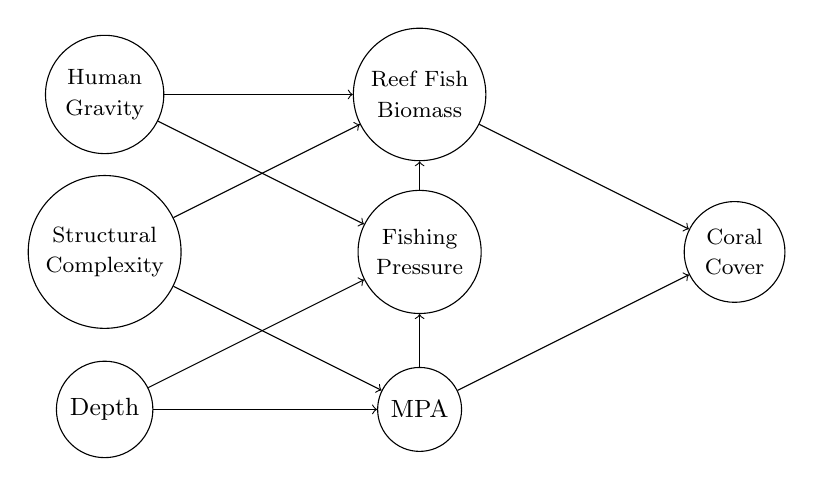
\begin{tikzpicture}
[every node/.style={font=\small, align = center}, every edge/.append style={nodes={font=\itshape\scriptsize}}]
\node (1) at (0,1) [shape=circle,draw] {Depth};
\node (2) at (0,3) [shape=circle,draw] {\footnotesize Structural\\
                                        \footnotesize Complexity};
\node (3) at (0,5) [shape=circle,draw] {\footnotesize Human\\
                                        \footnotesize Gravity};
\node (4) at (4,1) [shape=circle,draw] {MPA};
\node (5) at (4,3) [shape=circle,draw] {\footnotesize Fishing\\
                                        \footnotesize Pressure};
\node (6) at (4,5) [shape=circle,draw] {\footnotesize Reef Fish\\
                                        \footnotesize Biomass};
\node (7) at (8,3) [shape=circle,draw] {\footnotesize Coral\\
                                        \footnotesize Cover};
\draw [->] (1) edge (4);
\draw [->] (1) edge (5);
\draw [->] (2) edge (4);
\draw [->] (2) edge (6);
\draw [->] (3) edge (5);
\draw [->] (3) edge (6);
\draw [->] (4) edge (5);
\draw [->] (4) edge (7);
\draw [->] (5) edge (6);
\draw [->] (6) edge (7);
\end{tikzpicture}
\end{document}
